% !Tex program = pdflatex
% 第 7 章: 线性算子的结构 Chap 7: The Structure of a Linear Operator
\ifx\allfiles\undefined
\documentclass{note}
\setcounter{chapter}{+6}
\begin{document}
\fi
\chapter{线性算子的结构}
先来回顾一下\textbf{线性算子}: $V$ 为域 $F$ 上的向量空间, $\dim V=n$, $\mathcal{L}(V)=M_{n\times n}(F)$, $\dim\mathcal{L}(V)=n^2$,\\
取 $\forall\tau,\sigma\in\mathcal{L}(V)$, 有
\begin{itemize}
    \item[(1)] $(\tau+\sigma)(v)=\tau(v)+\sigma(v)$
    \item[(2)] $(\tau\circ\sigma)(v)=\tau(\sigma(v))$
    \item[(3)] $(r\tau)(v)=r\cdot\tau(v)$
\end{itemize}
其中 $\mathcal{L}(V)$ 关于 (1) 中的加法和 (2) 中的复合成环, 关于 (1) 中的加法和 (3) 中的点乘成向量空间, 故 $\mathcal{L}$ 为代数.\\
设 $\mathcal{B}=\{b_1,\cdots,b_n\}$, $\mathcal{B}'=\{b_1',\cdots,b_n'\}$ 分别是 $V$ 的两组定序基,
\begin{center}
    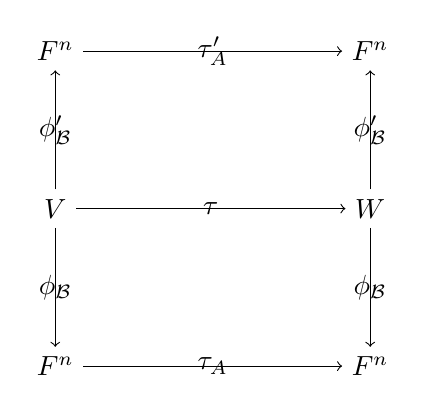
\begin{tikzpicture}
        \node(1)at(-2,0){$V$};
        \node(2)at(2,0){$W$};
        \node(3)at(-2,-2){$F^n$};
        \node(4)at(2,-2){$F^n$};
        \node(5)at(-2,2){$F^n$};
        \node(6)at(2,2){$F^n$};
        \draw[->](1)--(2)node[midway]{$\tau$};
        \draw[->](1)--(3)node[midway]{$\phi_{\mathcal{B}}$};
        \draw[->](2)--(4)node[midway]{$\phi_{\mathcal{B}}$};
        \draw[->](3)--(4)node[midway]{$\tau_A$};
        \draw[->](1)--(5)node[midway]{$\phi_{\mathcal{B}}'$};
        \draw[->](2)--(6)node[midway]{$\phi_{\mathcal{B}}'$};
        \draw[->](5)--(6)node[midway]{$\tau_A'$};
    \end{tikzpicture}
\end{center}

\begin{thm}[(课本定理 7.1)]
    线性算子 $\tau$ 在定序基 $\mathcal{B}$ 下的表示为 $[\tau]_{\mathcal{B}}=\begin{pmatrix}
        [\tau(b_1)]_{\mathcal{B}}&\cdots&[\tau(b_n)]_{\mathcal{B}'}
    \end{pmatrix}$.\\
    当 $\tau$ 作用于 $v\in V$, 可表为矩阵与向量相乘, $[\tau(v)]_{\mathcal{B}}=[\tau]_{\mathcal{B}}[v]_{\mathcal{B}}$.
\end{thm}

\begin{thm}[(课本定理 7.2)]
    $\tau$ 在两组定序基 $\mathcal{B}$ 和 $\mathcal{B}'$ 下的表示之间的关系是 $[\tau]_{\mathcal{B}'}=M_{\mathcal{BB}'}[\tau]_{\mathcal{B}}M_{\mathcal{BB}'}^{-1}$, 其中 $M_{\mathcal{BB}'}=\begin{pmatrix}
        [b_1]_{\mathcal{B}'}&\cdots&[b_n]_{\mathcal{B}'}
    \end{pmatrix}$.
\end{thm}

\begin{df}[相似]
    类似上面的 $[\tau]_{\mathcal{B}}$ 和 $[\tau]_{\mathcal{B}'}$, 若两个矩阵 $A,B$ 满足 $B=PAP^{-1}$, 则称 $A$ 与 $B$ \textbf{相似}, 由两两相似的矩阵组成的集合称为\textbf{相似类}.
\end{df}

取线性算子 $1,\tau,\tau^2,\cdots,\tau^{n^2}\in\mathcal{L}(V)$,\\
$\because$ 这些线性算子的数量 $n^2+1>\dim\mathcal{L}(V)=n^2$, $\therefore$ 这些线性算子线性相关,\\
即 $\exists$ 不全为 $0$ 的 $r_0,\cdots,r_{n^2}\in F$, s.t. $r_0+r_1\tau+\cdots+r_{n^2}\tau^{n^2}=0$\\
$\Longrightarrow\forall v\in V$, $\left(\sum_{i=0}^{n^2}r_i\tau^i\right)(v)=0\Longrightarrow\sum_{i=0}^{n^2}r_i\tau^i(v)=0$.\\
令 $f(x)=\sum_{i=0}^{n^2}r_ix^i\in\mathcal{L}(V)$, 则 $f(\tau)(v)=0$.

\begin{thm}[(课本定理 7.5)]
    $V$ 为域 $F$ 上的向量空间, 则 $V$ 为 $F[x]$ 上的模.
\end{thm}
\begin{pf}
    $\forall g(x)\in F[x]$, $g(x)$ 可表为 $g(x)=\sum_ia_ix^i$, 其中 $a_i\in F$, 则 $g(\tau)=\sum_ia_i\tau^i\in\mathcal{L}(V)$,\\
    $\forall h(x)\in F[x]$, $h(x)$ 可表为 $h(x)=\sum b_jx^j$, 其中 $b_j\in F$, 则 $h(\tau)=\sum_jb_j\tau^j\in\mathcal{L}(V)$,\\
    对于给定的 $\tau$, 有类似数乘的运算 $F[x]\times V\rightarrow V$, $(g(x),v)=g(x)\cdot v\mapsto g(\tau)(v)$, 满足
    \begin{itemize}
        \item[(1)] $[g(x)+h(x)]v=\left(\sum_ia_ix^i+\sum_jb_jx^j\right)v=\left(\sum_ia_i\tau^i+\sum_jb_j\tau^j\right)(v)=\left(\sum_ia_i\tau^i\right)(v)+\left(\sum_jb_j\tau^j\right)(v)=\left(\sum_ia_ix^i\right)v+\left(\sum_jb_jx^j\right)v=g(x)v+h(x)v$
        \item[(2)] $[g(x)h(x)]v=\left[\sum_ia_ix^i\sum_jb_jx^j\right]v=\left[\sum_ia_i\tau^i\circ\sum_jb_j\tau^j\right]v=\left(\sum_ia_i\tau^i\right)\left(\left(\sum_jb_j\tau^j\right)(v)\right)=\left(\sum_ia_ix^i\right)\left(\left(\sum_jb_jx^j\right)v\right)=g(x)[h(x)v]$
        \item[(3)] $g(x)(u+v)=\left(\sum_ia_ix^i\right)(u+v)=\left(\sum_ia_i\tau^i\right)(u+v)=\left(\sum_ia_i\tau^i\right)(u)+\left(\sum_ia_i\tau^i\right)(v)=\left(\sum_ia_ix^i\right)u+\left(\sum_ia_ix^i\right)v=g(x)v+g(x)u$
        \item[(4)] $1v=1(v)=v$
    \end{itemize}
    故 $V$ 为 $F[x]$ 上的模.
\end{pf}

$F[x]$ 为 PID, $V\in F[x]-\module$,\\
$\because\dim V=n$, $\therefore V$ 有限生成,\\
$\because f(x)v=f(\tau)(v)=0$, $\therefore V$ 为挠模,\\
利用定理 \ref{thm-6.11}, 可将 $V$ 分解为 $V=V_{p_1}\oplus\cdots\oplus V_{p_m}=\bigoplus_{i=1}^m\bigoplus_{j=1}^{t_i}\langle\langle v_{ij}\rangle\rangle$, 其中 $\ann(v_{ij})=\langle p^{e_{ij}}(x)\rangle$.

上面说明了分解 $V$ 的可行性和 $V$ 分解出的大致结构, 现在的问题是: 具体如何分解? 我们只要找到 $V$ 的阶 $\mu$, s.t. $\ann(V)=\langle\mu\rangle$, $\mu=up_1^{e_1}\cdots p_m^{e_m}$, 就可得到挠子模 $V_{p_i}$, s.t. $\ann(V_{p_i})=\langle p_i^{e_1}\rangle$ 及循环子模 $\langle\langle v_{ij}\rangle\rangle$, s.t. $\ann(v_{ij})=\langle p_i^{e_{ij}}\rangle$, $e_i\geq e_{i1}\geq\cdots\geq e_{it_i}$.

\begin{df}[极小多项式]
    $\ann(V)=\{g(x)\in F[x]\mid g(\tau)(V)=\{0\}\}=\langle m_{\tau}(x)\rangle$, 其中 $m_{\tau}(x)$ 称 $\tau$ 在 $V$ 上的\textbf{极小多项式}, 首系数 $=1$.
\end{df}

极小多项式就是 $V$ 的阶, 对其进行分解: $m_{\tau}(x)=up_1^{e_1}(x)\cdots p_n^{e_n}(x)$, 其中 $u$ 为单位, $p_i(x)\in F[x]$ 不可约且互不相等, $e_i\in\mathbb{Z}^+$,\\
$\Longrightarrow V=V_{p_1}\oplus\cdots\oplus V_{p_m}$, 其中 $\ann(V_{p_i})=\langle p_1^{e_1}(x)\rangle$,\\
$V_{p_i}=\langle\langle v_{i1}\rangle\rangle\oplus\cdots\oplus\langle\langle v_{it_i}\rangle\rangle$, 其中 $\ann(v_{ij})=\langle p_i^{e_{ij}}(x)\rangle$, $e_i\geq e_{i1}\geq\cdots\geq e_{it_i}$,\\
从而实现分解 $V=\bigoplus_{i=1}^m\bigoplus_{j=1}^{t_i}\langle\langle v_{ij}\rangle\rangle$.

接下来我们利用上述对 $V$ 的分解找一组合适的定序基, 以简化 $V$ 上的线性算子 $\tau$ 的表示.

\begin{df}[不变子空间]
    子空间 $S\subseteq V$, $\tau\in\mathcal{L}(V)$, 若 $\tau(S)\subseteq S$, 则称 $S$ 为 $V$ 的 $\tau$ \textbf{不变子空间}.
\end{df}

\begin{thm}[(课本定理 7.5)]
    子模 $S\subseteq V\Longleftrightarrow S$ 是 $V$ 的\textbf{不变子空间}.
\end{thm}
\begin{pf}
    ``$\Longrightarrow$'': $\forall v\in S\subseteq V$, $\forall h(x)\in F[x]$, $h(x)=\sum_ia_ix^i$, $h(x)v=h(\tau)(v)=\sum_ia_i\tau^i(v)\in S$,\\
    特别地, 取 $h(x)=x\in F[x]$, 则 $xv=\tau(v)\in S\Longrightarrow\tau(S)\subseteq S$, 即 $S$ 为 $V$ 的线性子空间.

    ``$\Longleftarrow$'': $\because S$ 是 $V$ 的不变子空间, $\therefore\forall v$, $\tau(v)\in S\Longrightarrow\forall i=0,\cdots,\dim V$, $\tau^i(v)\in S$,\\
    $g(x)v+h(x)v=g(\tau)(v)+h(\tau)(v)=\left(\sum_ia_i\tau^i\right)(v)+\left(\sum_jb_j\tau^j\right)(v)=\sum_i(a_i+b_i)\tau^i(v)\in S$, 故 $S$ 为 $V$ 的子模.
\end{pf}

$\because\langle\langle v_{ij}\rangle\rangle$ 为 $V$ 的 $F[x]$ 子模, $\therefore\langle\langle v_{ij}\rangle\rangle$ 为不变子空间, 即 $\tau(\langle\langle v_{ij}\rangle\rangle)\subseteq\langle\langle v_{ij}\rangle\rangle$, 故之前分解操作实际上是将 $V$ 分解成了一系列由单个向量生成的不变子空间.

让我们用简单的例子来展示一下, 若以不变子空间的基为整个向量空间的基 (的一部分), 线性算子的表示会如何.

\begin{eg}
    若 $\langle\langle b_1\rangle\rangle$ 是 $\tau$ 不变的, 则 $[\tau(b_1)]_{\mathcal{B}}=\begin{pmatrix}
        *\\
        0\\
        \vdots\\
        0
    \end{pmatrix}$, $[\tau]_{\mathcal{B}}=\begin{pmatrix}
        [\tau(b_1)]_{\mathcal{B}}&\cdots&[\tau(b_n)]_{\mathcal{B}}
    \end{pmatrix}=\begin{pmatrix}
        *&0&\cdots&0\\
        0\\
        \vdots\\
        0
    \end{pmatrix}$\footnote{$*$ 代表非零矩阵元.}\\
    若 $\langle\langle b_1,b_2\rangle\rangle$ 是 $\tau$ 不变的, 即 $\tau(b_1)\in\langle\langle b_1,b_2\rangle\rangle$, $\tau(b_2)\in\langle\langle b_1,b_2\rangle\rangle$, 则 $\begin{pmatrix}
        [\tau(b_1)]_{\mathcal{B}}&[\tau(b_1)]_{\mathcal{B}}
    \end{pmatrix}=\begin{pmatrix}
        *&*\\
        *&*\\
        0&0\\
        \vdots&\vdots\\
        0&0
    \end{pmatrix}$, $[\tau]_{\mathcal{B}}=\begin{pmatrix}
        *&*&0&\cdots&0\\
        *&*&0&\cdots&0\\
        0&0\\
        \vdots&\vdots\\
        0&0
    \end{pmatrix}$,\\
    若 $\langle\langle v_1,\cdots,v_k\rangle\rangle$ 是 $\tau$ 不变的, 则 $[\tau]_{\mathcal{B}}=\begin{pmatrix}
        *_{k\times k}&0\\
        0&\tau'
    \end{pmatrix}$.
\end{eg}

在之前我们已将 $V$ 分解成了多个不变子空间, 故若用各 $\langle v_{ij}\rangle$ 的基组成 $V$ 的基, 则可以将 $\tau$ 表示为一个仅在对角线上有非零矩阵块而其余部分均为零的矩阵. 但我们仍未满足: 对于给定的不变子空间 $\langle\langle v_{ij}\rangle\rangle$, 能否适当地选取该不变子空间中的基, 从而简化该不变子空间对应的非零矩阵块?

取 $\langle\langle v\rangle\rangle$ 的极小多项式为 $p(x)$ 即 $\ann(v)=\langle p(x)\rangle$, 设 $p(x)=x^m+r_{m-1}x^{m-1}+\cdots+r_1x+r_0$, $r_i\in F$,\\
则 $p(x)v=p(\tau)(v)=(\tau^m+r_{m-1}\tau^{m-1}+\cdots+r_1\tau+r_0)(v)=\tau^m(v)+r_{m-1}\tau^{m-1}(v)+\cdots+r_1\tau(v)+r_0v=0$,\\
即 $\tau^m(v)$ 可由 $\{v,\tau(v),\cdots,\tau^{m-1}(v)\}$ 线性表示: $\tau^m(v)=-\left[r_{m-1}\tau^{m-1}(v)+\cdots+r_1\tau(v)+r_0v\right]$,\\
$\Longrightarrow\tau^{m+1}(v)=\tau(\tau^m(v))=\tau(-\left[r_{m-1}\tau^{m-1}(v)+\cdots+r_1\tau(v)+r_0v\right])\\=-\left[r_{m-1}\tau^m(v)+r_{m-2}\tau^{m-1}(v)+\cdots+r_1\tau^2(v)+r_0\tau(v)\right]\\=-\left\{r_{m-1}\left[-r_{m-1}\tau^m(v)+\cdots+r_1\tau^2(v)+r_0\tau(v)\right]+r_{m-2}\tau^{m-1}(v)+\cdots+r_1\tau^2(v)+r_0\tau(v)\right\}$\\
易证, 任意高阶的 $\tau$ 作用于 $v$ 均可由 $\{v,\tau(v),\cdots,\tau^{m-1}(v)\}$ 线性表示, $\forall f(x)\in F[x]$ 作用于 $v$ 均可由 $\{v,\tau(v),\cdots,\tau^{m-1}(v)\}$ 线性表示.\\
由此, 我们引出:
\begin{thm}
    $\langle\langle v\rangle\rangle$ 为循环子模, 则 $\{v,\tau(v),\cdots,\tau^{m-1}(v)\}$ 是 $\langle\langle v\rangle\rangle$ 的基.
\end{thm}
\begin{pf}
    先证 $\{v,\tau(v),\cdots,\tau^{m-1}(v)\}$ 线性无关: 设 $l_0v+l_1\tau(v)+\cdots+l_{m-1}\tau^{m-1}(v)=0$,\\
    令 $h(x)=l_0+l_1x+\cdots+l_{m-1}x^{m-1}$, 则 $h(x)(v)\Longrightarrow h(x)\in\ann(v)=\langle p(x)\rangle\Longrightarrow p(x)\mid h(x)$,\\
    然而 $\because\deg p(x)=m\geq\deg h(x)=m-1$, $\therefore$ 只能有 $l_0=l_1=\cdots=l_{m-1}=0$, 故 $\{v,\tau(v),\cdots,\tau^{m-1}(v)\}$ 线性无关.

    再证 $\{v,\tau(v),\cdots,\tau^{m-1}(v)\}$ 生成 $\langle\langle v\rangle\rangle$: $\langle\langle v\rangle\rangle=\{h(x)v\mid h(x)\in F[x]\}=h(\tau)(v)$,\\
    $\forall h(\tau)v\in\langle\langle v\rangle\rangle$, 若$\deg h(x)\leq m-1$, 则 $h(x)v$ 显然可由 $\{v,\tau(v),\cdots,\tau^{m-1}\}$ 表示,
    若 $\deg h(x)\geq m-1$, 则 $h(x)=q(x)p(x)+r(x)$, 其中 $q(x)$ 为商多项式, 余多项式 $r(x)=0$ 或 $\deg r(x)<\deg p(x)=m-1$,\\
    $\Longrightarrow h(x)v=(q(\tau)p(\tau)+r(\tau))(v)=q(\tau)p(\tau)v+r(\tau)(v)$, 其中 $\because p(x)\in\ann(v)$, $\therefore p(\tau)v=0\Longrightarrow h(x)v=r(\tau)v$ 可由 $\{v,\tau(v),\cdots,\tau^{m-1}\}$ 表示.

    综上, 得证.
\end{pf}

\begin{df}[循环不变子空间]
    $S$ 是向量空间 $V$ 的 $\tau$ 不变子空间, 若 $S$ 有一组基 $\mathcal{B}=\{v,\tau(v),\cdots,\tau^{m-1}(v)\}$, 其中 $v\in V$, $m\geq 1$, 则称 $S$ 是 $V$ 的\textbf{循环不变子空间}.
\end{df}

$\langle\langle v_{ij}\rangle\rangle$ 就是循环不变子空间. 那么, 以 $\mathcal{B}_{ij}=\{v_{ij},\tau(v_{ij}),\cdots,\tau^{m-1}(v_{ij})\}$ 为基, 线性算子 $\tau$ 在该循环不变子空间中的表示 (即 $\tau$ 的表示中该循环不变子空间对应的非零矩阵块) 如何?

% \begin{thm}[(课本定理 7.7)]
%     $V$ 为有限维向量空间, $S\subseteq V$,\\
%     $S$ 为 $V$ 的循环子模, $\ann(S)=\langle p(x)\rangle$, $\deg p(x)=m$ $\Longleftrightarrow S$ 是 $V$ 的 $\tau$ 不变子空间.
% \end{thm}

\begin{df}[伴阵]
    在定序基 $\mathcal{B}=\{v,\tau(v),\cdots,\tau^{m-1}(v)\}$ 下, 线性算子 $\tau$ 可表为 $[\tau]_{\mathcal{B}}=\begin{pmatrix}
            [\tau(b_1)]_{\mathcal{B}}&\cdots&[\tau(b_m)]_{\mathcal{B}}
    \end{pmatrix}$,\\
    其中 $[\tau(b_1)]_{\mathcal{B}}=[\tau(v)]_{\mathcal{B}}=\begin{pmatrix}
        0\\
        1\\
        0\\
        \vdots\\
        0
    \end{pmatrix}$, $[\tau(b_2)]_{\mathcal{B}}=[\tau(\tau(v))]_{\mathcal{B}}=[\tau^2(v)]_{\mathcal{B}}=\begin{pmatrix}
        0\\
        0\\
        1\\
        0\\
        \vdots\\
        0
    \end{pmatrix}$, $\cdots$, $[\tau(b_m)]_{\mathcal{B}}=[\tau^m(v)]_{\mathcal{B}}=\begin{pmatrix}
        -r_0\\
        -r_1\\
        \vdots\\
        -r_{m-1}
    \end{pmatrix}$,\\
    从而 $[\tau]_{\mathcal{B}}=\begin{pmatrix}
        0&0&\cdots&0&-r_0\\
        1&0&\cdots&0&-r_1\\
        0&1&\cdots&0&-r_2\\
        0&0&\cdots&0&-r_3\\
        \vdots&\vdots&\ddots&\vdots&\vdots\\
        0&0&\cdots&0&-r_{m-2}\\
        0&0&\cdots&1&-r_{m-1}
    \end{pmatrix}\equiv C[p(x)]$, 称为多项式 $p(x)=x^m+r_{m-1}x^{m-1}+\cdots+r_1x+r_0$ 的\textbf{伴阵}.
\end{df}

设 $d_{ij}=\deg p_i^{e_{ij}}(x)$, 则 $\mathcal{B}_{ij}=\{v_{ij},\tau(v_{ij}),\cdots,\tau^{d_{ij}-1}(v_{ij})\}$ 为 $\langle v_{ij}\rangle$ 的基,\\
以 $\mathcal{B}_{ij}$ 为基, $\tau$ 在循环不变子空间 $\langle\langle v_{ij}\rangle\rangle$ 中的表示就是 $p_i^{e_{ij}}(x)$ 的伴阵: $[\tau]_{\mathcal{B}_{ij}}=C[p_i^{e_{ij}}(x)]=\begin{pmatrix}
    0&0&\cdots&0&-l_1^{(ij)}\\
    1&0&\cdots&0&-l_2^{(ij)}\\
    0&1&\cdots&0&-l_3^{(ij)}\\
    0&0&\cdots&0&-l_4^{(ij)}\\
    \vdots&\vdots&\ddots&\vdots&\vdots\\
    0&0&\cdots&0&-l_{d_{ij}-2}^{(ij)}\\
    0&0&\cdots&1&-l_{d_{ij}-1}^{(ij)}
\end{pmatrix}$.\\

上面我们简化了 $\tau$ 在循环不变子空间 $\langle\langle v_{ij}\rangle\rangle$ 中的表示. 又 $\because V=\bigoplus_{ij}\langle\langle v_{ij}\rangle\rangle$, $\therefore\mathcal{B}=\cup_{ij}\mathcal{B}_{ij}$ 为 $V$ 的基, 利用 $\mathcal{B}$ 我们可简化 $\tau$ 在整个向量空间 $V$ 中的表示:
\begin{thm}[(课本定理 7.10)]
    $\dim V<\infty$, $\tau\in\mathcal{L}(V)$, $V$ 的极小多项式为 $m_{\tau}(x)=p_1^{e_1}(x)\cdots p_n^{e_n}(x)$, 其中 $p_i(x)$ 不可约且互不相等,\\
    $\Longrightarrow V=V_{p_1}\oplus\cdots\oplus V_{p_m}$, 其中 $\ann(V_{p_i})=\langle p_1^{e_1}(x)\rangle$,\\
    $V_{p_i}=\langle\langle v_{i1}\rangle\rangle\oplus\cdots\oplus\langle\langle v_{it_i}\rangle\rangle$, 其中 $\ann(v_{ij})=\langle p_i^{e_{ij}}(x)\rangle$, $e_i\geq e_{i1}\geq\cdots\geq e_{it_i}$,\\
    以 $\cup_{ij}\{v_{ij},\tau(v_{ij}),\cdots,\tau^{d_{ij}-1}(v)\}$ 为基, 其中 $d_{ij}=\dim\langle\langle v_{ij}\rangle\rangle$, $\tau$ 的表示可简化为
    $$[\tau]_{\mathcal{B}}=\begin{pmatrix}
        C[p_1^{e_{11}}(x)]\\
        &\ddots\\
        &&C[p_1^{e_{1t_1}}(x)]\\
        &&&\ddots\\
        &&&&C[p_m^{e_{m1}}(x)]\\
        &&&&&\ddots\\
        &&&&&&C[p_m^{e_{mt_m}}(x)]
    \end{pmatrix}.$$
\end{thm}

\begin{df}[有理标准型]
    上述线性变换的矩阵表示称为\textbf{有理标准型}.
\end{df}

$n=\dim V=\sum_{ij}d_{ij}=\sum_{ij}\deg p_i^{e_{ij}}(x)=\deg\left[\prod_{ij}p_i^{e_{ij}}(x)\right]$.
\ifx\allfiles\undefined
\end{document}
\fi